\documentclass{beamer}
\usepackage{listings}
\lstset{
%language=C,
frame=single, 
breaklines=true,
columns=fullflexible
}
\usepackage{blkarray}
\usepackage{subcaption}
\usepackage{url}
\usepackage{tikz}
\usepackage{tkz-euclide} % loads  TikZ and tkz-base
%\usetkzobj{all}
\usetikzlibrary{calc,math}
\usepackage{float}
\newcommand\norm[1]{\left\lVert#1\right\rVert}
\renewcommand{\vec}[1]{\mathbf{#1}}
\usepackage[export]{adjustbox}
\usepackage[utf8]{inputenc}
\usepackage{amsmath}
\usepackage{amsfonts}
\usepackage{tikz}
\usepackage{hyperref}
\usepackage{bm}
\hypersetup{
    colorlinks = true,
    linkbordercolor = {white},
    linkcolor={red},
    citecolor={green},
    filecolor={blue},
	menucolor={red},
	runcolor={cyan},
	urlcolor={blue},
	breaklinks=true
}
\usetikzlibrary{automata, positioning}
\usetheme{Boadilla}
\providecommand{\pr}[1]{\ensuremath{\Pr\left(#1\right)}}
\providecommand{\mbf}{\mathbf}
\providecommand{\qfunc}[1]{\ensuremath{Q\left(#1\right)}}
\providecommand{\sbrak}[1]{\ensuremath{{}\left[#1\right]}}
\providecommand{\lsbrak}[1]{\ensuremath{{}\left[#1\right.}}
\providecommand{\rsbrak}[1]{\ensuremath{{}\left.#1\right]}}
\providecommand{\brak}[1]{\ensuremath{\left(#1\right)}}
\providecommand{\lbrak}[1]{\ensuremath{\left(#1\right.}}
\providecommand{\rbrak}[1]{\ensuremath{\left.#1\right)}}
\providecommand{\cbrak}[1]{\ensuremath{\left\{#1\right\}}}
\providecommand{\lcbrak}[1]{\ensuremath{\left\{#1\right.}}
\providecommand{\rcbrak}[1]{\ensuremath{\left.#1\right\}}}
\providecommand{\abs}[1]{\vert#1\vert}

\newcounter{saveenumi}
\newcommand{\seti}{\setcounter{saveenumi}{\value{enumi}}}
\newcommand{\conti}{\setcounter{enumi}{\value{saveenumi}}}

\makeatletter
\newenvironment<>{proofs}[1][\proofname]{%
    \par
    \def\insertproofname{#1\@addpunct{.}}%
    \usebeamertemplate{proof begin}#2}
  {\usebeamertemplate{proof end}}
\makeatother

\title{Research Paper Presentation - RP 12}
\author{Anirudh Srinivasan}
\institute{IIT Hyderabad}
\date{CS20BTECH11059}
\begin{document}

\begin{frame}
\titlepage
\end{frame}

\begin{frame}
\frametitle{Title and Authors}
\begin{block}{Title}
A Performance Comparison of Data Mining Algorithms Based Intrusion Detection System for Smart Grid
\end{block}
\begin{block}{Authors}
\begin{enumerate}
\item Zakaria El Mrabet, School of Electrical Engineering \& Computer Science, University of North Dakota, USA 
\item Hassan El Ghazi, National Institute of Posts \& Telecommunication, Rabat, Morocco
\item Naima Kaabouch, School of Electrical Engineering \& Computer Science, University of North Dakota, USA
\end{enumerate}
\end{block}
\end{frame}

\begin{frame}{Abstract}
\begin{enumerate}
\item Smart grid is an emerging and promising technology. It uses the power of information technologies to deliver intelligently the electrical power to customers.
\item Unfortunately, information technologies have inherent vulnerabilities and weaknesses that expose the smart grid to a wide variety of security risks.
\item Intrusion detection system (IDS) plays an important role in securing smart grid networks and detecting malicious activity, yet it suffers from several limitations.
\item This paper presents an overview of four data mining algorithms used by IDS in Smart Grid. 
\end{enumerate}
\end{frame}

\begin{frame}{Key Concepts and Definitions}
\begin{itemize}

\item \textbf{Smart Grid} : It is an electricity network enabling a two-way flow of electricity and data with digital communications technology enabling to detect, react and pro-act to changes in usage and multiple issues. Smart grids have self-healing capabilities and enable electricity customers to become active participants.
\item \textbf{IDS} : It is a device or software application that monitors a network for malicious activity or policy violations.
\item \textbf{Data Mining Algorithms} : These are a set of heuristics and calculations that creates a model from data. Optimal parameters for creating the mining model is found on analysing and these are then applied across the entire data set to extract actionable patterns and detailed statistics.

\end{itemize}
\end{frame}



\begin{frame}{Introduction}
\begin{enumerate}
\item Compared to the traditional power grid, smart grid provides
new functionalities such as real-time control, two-way flow of
information communication, operational efficiency, and grid
resilience.
\item IDS is based on three distinct approaches in detecting
abnormalities:
\begin{itemize}
    \item Signature-based: Detects patterns of malicious activities using a database of well-known attack signatures
    \item Specification-based: Identifies deviation from normal behavior profiles using logical specifications
    \item Anomaly-based: Looks for deviations from normal behavior profiles using statistical measures
\end{itemize}
\item The anomaly-based technique is more applicable and suitable approach for smart grid than signature-based and specification-based techniques.
\seti 
\end{enumerate}
\end{frame}

\begin{frame}{Introduction Contd.}
\begin{enumerate}
\conti
\item Despite its wide use, IDS suffers from several performance limitations, including limited detection accuracy and high rate of false positive.
\item This paper evaluates the performance of 4 Data mining algorithms used in IDS, which are: 
\begin{itemize}
    \item Naïve Bayes
    \item Decision tree
    \item Support Vector Machine, and 
    \item Random Forest
\end{itemize}
\item The benchmark NSL-KDD (Network Security Laboratory - Knowledge Discovery in Databases) dataset is selected for this evaluation
\item The evaluation is based on the following metrics:
\begin{itemize}
    \item Probability of detection or true positive rate (TPR)
    \item Probability of false alarm or false positive rate (FPR)
    \item Probability of miss detection or false negative rate (FNR)
    \item Efficiency and Processing time.
\end{itemize} 
\end{enumerate}
\end{frame}

\begin{frame}{Naive Bayes}
\begin{enumerate}
\item When the features/attributes of the data are independent, we can extend the Bayes Rule to what is called Naive Bayes, whose name is based on the naive assumption that the X’s are independent of each other
\item \textbf{Bayes Rule:}
\begin{align}
    \pr{Y|X} = \frac{\pr{X|Y}\times\pr{Y}}{\pr{X}}
\end{align}
\item \textbf{Naive Bayes Rule:}
\begin{multline}
        \pr{Y=k|X_1\dots X_2} = \\\frac{\pr{X_1|Y=k} \times \pr{X_2|Y=k}\dots \pr{X_n|Y=k}\times\pr{Y}}{\pr{X_1} \times \pr{X_2}\dots \pr{X_n}}
\seti
\end{multline}


\end{enumerate}
\end{frame}

\begin{frame}{Naive Bayes Contd.}
\begin{enumerate}
\conti
\item Let D be a training set of a tuple and their associated
class labels. In our case, a tuple is a packet and it is
represented by an n-dimensional attribute vector X =
\{$x_1, x_2, x_3,…, x_n$\}.
\item The number of classes = m = 2 (attack
class, normal class). Given a tuple or a packet X,
NB will predict that X belongs to the class with the
highest posterior probability. In other words, X
belongs to $C_i$ if and only if:
\begin{align}
\pr{C_i|X} > \pr{C_j|X} \text{ for } 1 \leq j \leq m, i \neq j
\end{align}

\seti
\item \begin{align}
\pr{C_i} = \frac{|C_{i,D}|}{|D|}
\end{align}
where: $|C_{i,D}|$ is the number of training tuple of class $C_i$ in
D.
\seti
\end{enumerate}
\end{frame}

\begin{frame}{Naive Bayes Contd.}
\begin{enumerate}
\conti
\item As NB assumes that there is no relationship among
child nodes or attributes, the \pr{X|Ci} is given by:
\begin{align}
    \pr{X|C_i} = \pr{x_1|C_i}\times \pr{x_2|C_i}\dots \pr{x_n|C_i}
\end{align}
where: $x_k$ is the value of attribute $A_k$ for tuple X. 
\item As the attributes $A_1,A_2,\dots A_n$ in the data set are categorical, we have:
\begin{align}
    \pr{x_k|C_i} = \frac{|C_{i,D,x_k}|}{|C_{i,D}|}
\end{align} 
where: $|C_{i,D,x_k}|$ is the number of tuples of class $C_i$ in D having the value $x_k$ for $A_k$
\seti
\end{enumerate}
\end{frame}

\begin{frame}{Decision Tree Algorithm}
\begin{enumerate}
\item The decision tree is a supervised learning algorithm that
can be used for addressing the classification problem. It
consists of root node, branches nodes, and leaf nodes. 
\item Each node represents a feature or attribute. Each link or branch represent a decision or rule and the leaf node is the class label to which a given object belongs.
\item \textbf{Entropy:} It is a measure of uncertainity in the dataset
\begin{align}
    S(D) = \frac{-p}{p+n} \log_{2}\left(\frac{p}{p+n}\right) - \frac{n}{p+n} \log_{2}\left(\frac{n}{p+n}\right)
\end{align}
where: p is the number of positive examples and n is the number of negative examples in the dataset.
\item \textbf{Average information entropy:} 
\begin{align}
    I(A_k) = \sum_{\forall i} \frac{p_i+n_i}{p+n} \times S(A_k = x_i)
\end{align}


\seti
\end{enumerate}
\end{frame}

\begin{frame}{Decision Tree Algorithm Contd}
\begin{enumerate}

\conti
\item \textbf{Information Gain:} It is a measure of how much information the answer to a specific question provides. It is the difference in entropy before and after splitting the dataset on attribute A.
\begin{align}
    G(A_k) = S(D) - I(A_k)
\end{align}
\item The attribute that best classifies the training data should be used as the root node of the tree.
\item \textbf{Algorithm:}
\begin{itemize}

\item Compute the entropy of the entire dataset
\item For every attribute or feature:
\begin{itemize}
    \item Calculate entropy for all the values that the particular attribute can take
    \item Calculate average information entropy for the current attribute
    \item Calculate gain for the current attribute
\end{itemize}
\item Pick the attribute with highest gain for this node
\item Repeat until we get a complete decision tree with leaf nodes at the end.
\seti
\end{itemize}

\end{enumerate}
\end{frame}

\begin{frame}{Support Vector Machine}
\begin{enumerate}
\item SVM is a machine learning algorithm used for
classification and regression. It is based on a hyper line
classifier, which separates and maximizes the margin between
two classes 
\item Let the data set D be given as \{$(x_1, y_1),(x_2, y_2),(x_3, y_3),...,(x_N,y_N)$\} where $x_i$ is the set of training tuples with associated class label $y_i$. Each $y_i$ can take one of two values, either +1 or -1, corresponding to the class ‘attack’ and class ‘normal’.
\item SVM finds the best decision boundary to separate two
classes by searching for the maximum margin hyper line. A separating hyper line can be written as:
\begin{align}
    h(x) = \omega^TX + b
\end{align}
\seti
\end{enumerate}
\end{frame}

\begin{frame}{Support Vector Machine Contd.}
\begin{figure}[ht]
    \centering
    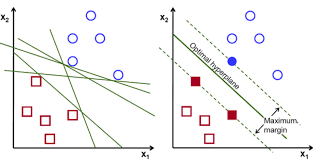
\includegraphics[width=0.5\textwidth]{SVM.png}
    \caption{Diagram illustrating Support Vector Machines}
    \label{SVM}
\end{figure}
\begin{enumerate}
\conti    
\item 
For all the red colored points, h(x) is positive and is taken to be 1 after normalization, since it is a classification problem. Similarly, for all blue coloured points h(x) is negative and it taken to be -1.
\seti
\end{enumerate}
\end{frame}

\begin{frame}{Support Vector Machine Contd.}
\begin{enumerate}
\conti
\item To find the optimum hyperplane, we have to find ($\omega$,b) so as to:
\begin{align}
    \text{Maximize } \frac{2}{||\omega||} \text{ such that } y_i\times (\omega^TX + b) \geq 1
\end{align}

\item In order to create a generalised model, the cost function for this algorithm can be given by:
\begin{align}
    J(\omega,b) = \frac{||\omega||}{2} + c_i \sum_{i=1}^n \epsilon_i
\end{align}
where: $c_i$ = Number of permissible errors, which is also called regularization parameter and $\epsilon_i$ = value of errors
\end{enumerate}
\end{frame}

\begin{frame}{SVM Kernels}
 \begin{enumerate}
    \item In the case of non-linear data, we can first transform the
data through non-linear mapping to another higher dimension
space and then use a linear model to separate the data. The
mapping function is done by a kernel function
\end{enumerate}
\begin{figure}[ht]
    \centering
    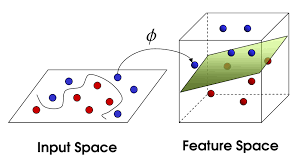
\includegraphics[width=0.5\textwidth]{SVM_Kernels.png}
    \caption{Diagram illustrating SVM Kernels}
    \label{SVM_Kernels}
\end{figure}
\end{frame}  

\begin{frame}{Random Forest}
 \begin{enumerate}
     \item RF is a classifier which induces an ensemble of randomized decision trees for classification and
prediction. Randomness is achieved either by selecting a
 sample from the training data set or by selecting randomly a subset of attribute at each node of each decision tree. 
 \item It has low bias and low variance unlike a normal decision tree algorithm which has low bias and high variance while predicting the class of test data.
 \begin{figure}[ht]
    \centering
    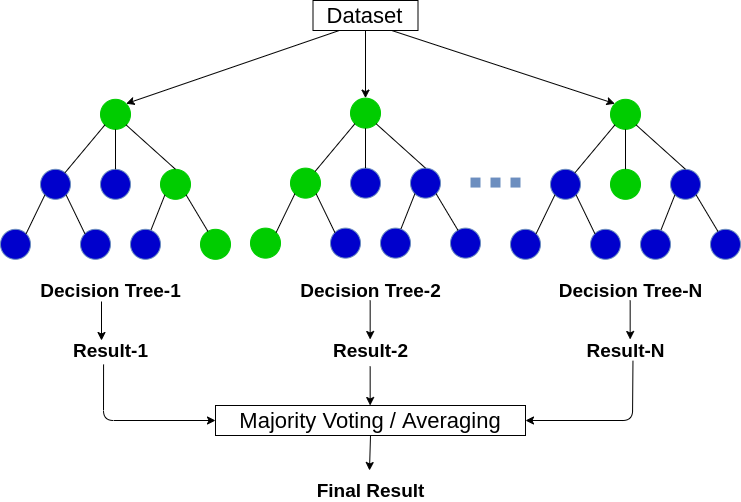
\includegraphics[width=0.5\textwidth]{RFC.png}
    \caption{Diagram illustrating Random Forest Classifier}
    \label{RFC}
\end{figure}
 \end{enumerate}
\end{frame}

\begin{frame}{NSL-KDD Dataset}
\begin{enumerate}
    \item Although KDD Cup 99 is considered as a benchmark data
set for assessing anomaly detection algorithms, it has a large
number of redundant connections, especially a repeating
record of DOS category. 
    \item In addition, there is a bias distribution of the four categories which makes an accurate classification of the U2R and R2L difficult. These issues have been addressed in the NSL-KDD data set.

\begin{center}
\begin{table}[h]
    \centering
    \scalebox{0.8}{
    \resizebox{\columnwidth}{!}{
\begin{tabular}{|c|c|c|}
\hline
\textbf{Attack’s category}     & \textbf{Description }                                                                & \textbf{Attack’s Examples}                \\ \hline
Remote to Local (R2L) & Unauthorized access from a remote machine                                   & Password guessing                \\ \hline
User to Root (U2R)    &  \begin{tabular}{@{}c@{}}Unauthorized access to local root privileges \\ from a local unprivileged user\end{tabular} & \begin{tabular}{@{}c@{}}Rootkits,  \\ buffer overflow attack\end{tabular}\\ \hline
DOS                   & Denial of service                                                           & \begin{tabular}{@{}c@{}}Teardrop attack and  \\  Smurf attack \end{tabular}\\ \hline
Probing               & Surveillance and scanning                                                   & Scanning attack                  \\ \hline
\end{tabular}
}
}
    \caption{Attack’s categories in KDD CUP 99 and NSL-KDD}
    \label{Attack categories table}
\end{table}
\end{center}
\end{enumerate}

\end{frame}

\begin{frame}{Comparison of the 4 Algorithms}
\begin{enumerate}
    \item The probability of detection or true positive rate (TPR) is given by:
\begin{align} 
    TPR = \frac{TP}{TP+FN} \times 100
\end{align}

    \item The probability of false alarm or false positive rate (FPR) is given by:
\begin{align}
    FPR = \frac{FP}{FP+TN} \times 100
\end{align}
    
    \item The probability of miss detection or false negative rate (FNR) is given by:
  \begin{align}
    FNR = \frac{FN}{TP+FN} \times 100
\end{align}  

\item The efficiency or accuracy is given by:
  \begin{align}
    \text{Efficiency } = \frac{TP+TN}{TP+TN+FP+FN} \times 100
\end{align}  
\textbf{where:} TP = True Positive, FP = False Positive, TN = True Negative, FN = False Negative
\end{enumerate}   
\end{frame}

\begin{frame}{Results}
     \begin{figure}[ht]
    \centering
    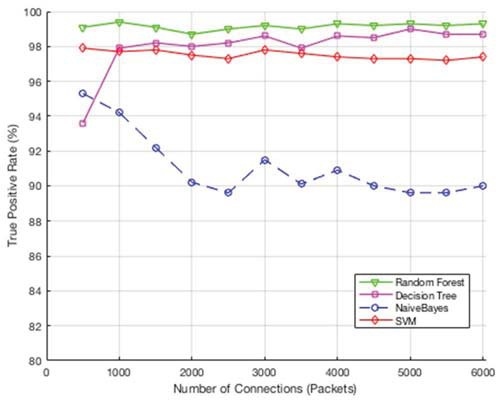
\includegraphics[width=0.32\textwidth]{TPR.jpeg}
    \caption{TPR vs Number of Packets}
    \label{TPR}
\end{figure}
    \begin{figure}[ht]
    \centering
    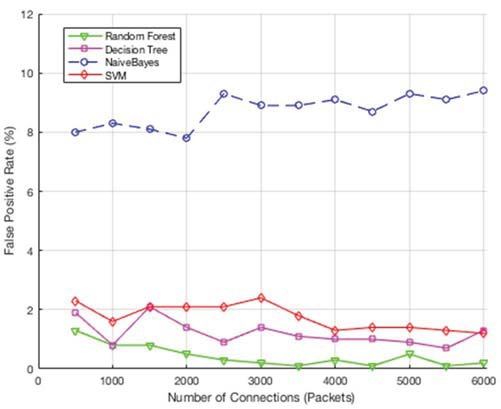
\includegraphics[width=0.32\textwidth]{FPR.jpeg}
    \caption{FPR vs Number of Packets}
    \label{FPR}
\end{figure}
\end{frame}

\begin{frame}{Results Contd.}
        \begin{figure}[ht]
    \centering
    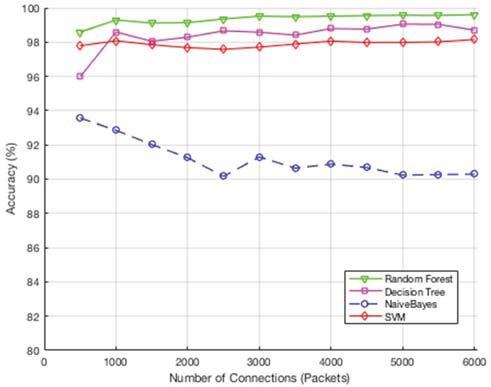
\includegraphics[width=0.32\textwidth]{Accuracy.jpg}
    \caption{Accuracy vs Number of Packets}
    \label{Accuracy}
\end{figure} 
\begin{figure}[ht]
    \centering
    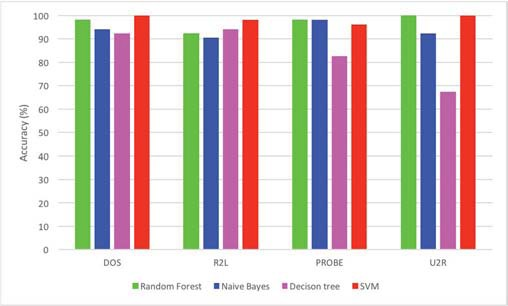
\includegraphics[width=0.32\textwidth]{Accuracy_Attack.jpeg}
    \caption{Accuracy vs Attack's category}
    \label{Accuracy}
\end{figure} 
\end{frame}

\begin{frame}{Conclusions and Future Work}
\begin{enumerate}
    \item Random Forest is better than the other three algorithms in classifying attacks with a higher probability of detection, lower probability of false alarm, lower probability of miss detection, and higher accuracy
    \item It detects most of the attack including DOS,
PROBE, and U2R attacks. However, its main drawback is that
it is time-consuming.
    \item On the other hand, Naïve Bayes shows
the lowest probability of detection, highest probability of false
alarm, the highest probability of miss detection, and lowest
accuracy; but, it requires less processing time than the three
other algorithms.
\item As future work, we aim to
develop algorithms that satisfy the tradeoff between
processing time and accuracy.
\end{enumerate}
      
\end{frame}
\end{document}